%!TEX ROOT=formularioFisica.tex

\section{Idrostatica}
L'idrostatica studia i fluidi in stato di equilibrio. Studia anche le pressioni.
\subsection{Legge di Stevino}
La legge di Stevino trova la pressione ad una data profondit�.
\begin{equation*}
p = p_{atm} + \delta gh
\end{equation*}
$\delta$: densit� del liquido\\
\hyperref[tab:patm]{$p_{atm}$}: $1\,\text{atm} = 1.01\cdot10^5\,\text{Pa} = 760\,\text{mm\,Hg} = 
1.01\cdot10^5\,\text{N/m}^2 = 1\,\text{bar}$\\
\hyperref[tab:g]{$g$}: $9.81\,\text{m/s}^2$\\
$h$: profondit�\\[\baselineskip]
Se vista in un modo pi� generale si trova la pressione tra due punti
\begin{equation*}
p_2 = p_1 + \delta g\Delta h
\end{equation*}
$\delta$: densit� del liquido\\
\hyperref[tab:g]{$g$}: $9.81\,\text{m/s}^2$\\
$h$: profondit�\\ [\baselineskip]

Si ricordi che $\text{Densit�}=\frac{\text{Massa}}{\text{Volume}}$.

\subsection{Torchio idraulico}
\begin{center}
	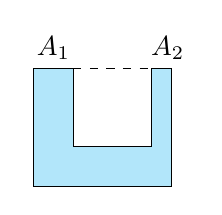
\begin{tikzpicture}
		\filldraw[cyan, fill opacity = 0.3]
		(0,0) -- ++(0.5,0) -- ++(0,-1) -- ++(1,0) -- ++(0,1) -- ++(0.25,0) --
		++(0,-1.5) -- ++(-1.75,0) -- ++(0,1.5);
		\draw 
		(0,0) -- ++(0.5,0) -- ++(0,-1) -- ++(1,0) -- ++(0,1) -- ++(0.25,0) --
		++(0,-1.5) -- ++(-1.75,0) -- ++(0,1.5);
		\draw[dashed] (0.5,0) -- +(1,0);
		\node at (0.25,0.25){$A_1$};
		\node at (1.7,0.25){$A_2$};
	\end{tikzpicture}
\end{center}
Il torchio idraulico permette partendo da una forza applicata su un pistone (di area $A_1$) di ottenere
una forza pi� grande su un altro pistone (di area $A_2$).
\begin{equation*}
p = \frac{F}{A}\qquad \frac{F_1}{A_1}=\frac{F_2}{A_2}
\end{equation*}

\subsection{Principio di Pascal}
Il principio di Pascal afferma che in un liquido  una pressione che venga esercitata in un punto  
viene trasmessa a ogni suo altro punto e in ogni sua direzione.

\subsection{Legge dei vasi comunicanti}
\begin{equation*}
\frac{h_1}{h_2} = \frac{\delta_2}{\delta_1}
\end{equation*}
I livelli di liquidi sono inversamente proporzionali alla densit� dei liquidi. Si presti attenzione
alla densit� corretta.

\subsection{Principio di Archimede}
Il principio di Archimede permette di trovare la forza di galleggiamento.
\begin{equation*}
F_g = \delta_fVg
\end{equation*}
Al principio di Archimede � collegata la condizione di equilibrio di un corpo in un fluido:\\
\begin{center}
	\emph{`Un corpo � in equilibrio in un fluido se la sua forza peso compensa la spinta di 
		Archimede, cio� se il suo peso � uguale al peso del fluido spostato.'}
\end{center}

\subsection{Volume della parte immersa}
\begin{equation*}
V_{imm} = V_s\frac{\delta_s}{\delta_f}
\end{equation*}
$_s$: relativo al solido\\
$_f$: relativo al fluido